
\chapter{Infraestructura}
En esta sección describiremos la infraestructura que hemos construido para el desarrollo del proyecto.
\section{Repositorio GIT}
\label{sect:repositorio}
El código del proyecto, así como las presentaciones y memoria de este proyecto, está almacenado en el 
repositorio \url{https://github.com/MaiteMartinez/MBITProject_Data4all}

\myfigure{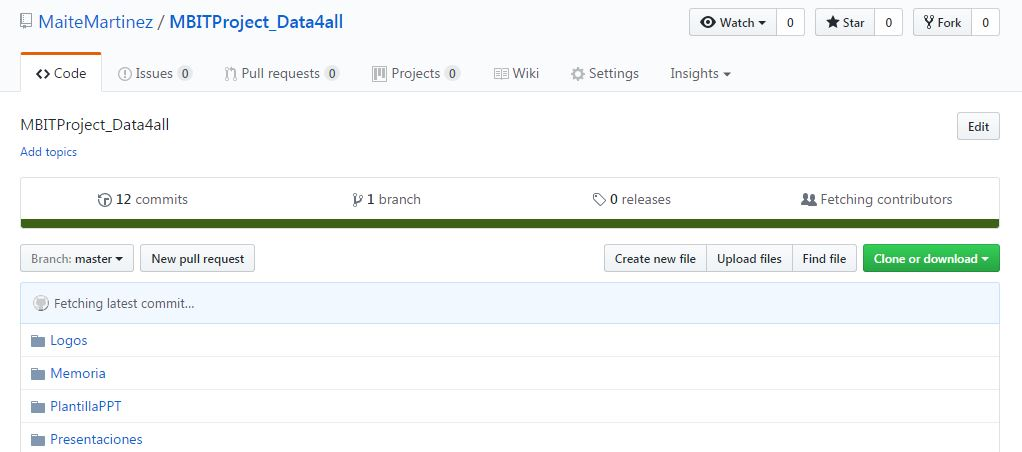
\includegraphics[width=0.6\textwidth]{repositorio_git1}%
\figcaption{Repositorio del código del proyecto.}
\label{fig:repositorio_git1} }

\section{Infraestructura para la obtención de datos}

Como muchas redes sociales, Twitter ofrece acceso a la información que generan sus usuarios a través de un
API ({\em Application Programming Interface})\cite{twitter_dev_web}. El API de Twitter ofrece diversas opciones: 
Webhook APIs, ADS API, REST APIs y Streaming APIs. La primera está enfocada a generar  
notificaciones instantáneas a partir de detección de eventos y la segunda a la integración de aplicaciones con la 
plataforma de publicidad de Twitter. Para nuestro proyecto, solo son relevantes por tanto las dos segundas:
\begin{itemize}
\item El API Rest ({\em Representational State Transfer}) permite realizar consultas puntuales con los parámetros de búsqueda indicados,
a través de una componente denominada Search API. El Search API funciona de manera similar, aunque no 
exactamente igual, a la búsqueda en la página web de Twitter. El Search API 
realiza la búsqueda entre una muestra de tuits publicados en los últimos siete días, y
las búsquedas están limitadas a 180 peticiones cada ventana temporal de 15 minutos. 

\myfigure{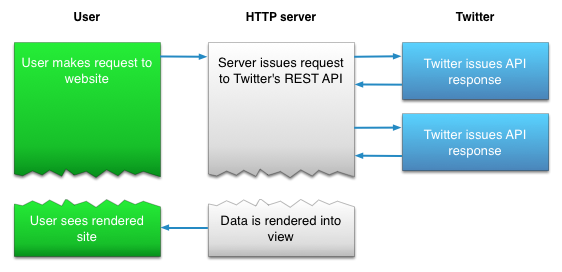
\includegraphics[width=0.6\textwidth]{api_rest_como_funciona}%
\figcaption{Funcionamiento del API Rest. \url{ https://dev.twitter.com/streaming/overview}}
\label{fig:api_rest_como_funciona} }

La búsqueda realizada por este API está centrada en la relevancia y no en la completitud, lo que 
quiere decir que algunos tuits y usuarios podrían quedarse fuera.

\item El API Streaming permite un acceso con baja latencia al flujo global de tuits de la aplicación,
y requiere una conexión HTTP continua. Entre los tipos de flujos disponibles, en la web de Twitter
para desarrolladores, se recomienda usar los flujos públicos para realizar minería de datos (en dichos flujos
aparecen muestras de los datos públicos de Twitter).

\myfigure{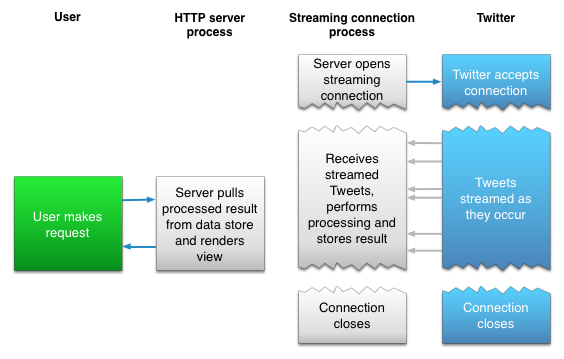
\includegraphics[width=0.6\textwidth]{api_streaming_como_funciona}%
\figcaption{Funcionamiento del API Streaming. \url{ https://dev.twitter.com/streaming/overview}}
\label{fig:api_streaming_como_funciona} }

\end{itemize}

El acceso a ambas versiones de API está gobernado por la autentificación mediante el protocolo OAuth
({\em Open Authorization}), lo que implica que para cada aplicación deben obtenerse los tokens necesarios 
de la sección de desarrolladores de Twitter, estableciéndose un número máximo de 7 por usuario.
También para ambas versiones del API existen restricciones de acceso. Estas restricciones solo
afectan a las versiones gratuitas de los APIs. Hay una versión de pago de este acceso  (Twitter Firehose)
que garantiza como respuesta el 100\% de los tuits que cumplan los criterios de la búsqueda.
Para el desarrollo de este proyecto nos hemos servido del API gratuito, por limitación de costes. 

Entre los API REST y Streaming, hemos decidido utilizar el API Streaming, mediante un script
en Python usando {\tt Tweepy}. Este método tiene diversas ventajas y desventajas que pasamos
a revisar:
\begin{enumerate}
\item El API Streaming proporciona tuits en tiempo real, y funciona como una especie de \lq\lq grabadora\rq\rq,
con la que se van registrando todos los tuits a medida que se van produciendo.
\item Como es un proceso que se mantiene a la escucha y va reflejando entradas según
se producen, la infraestructura necesaria para que funcione es algo  más complicada que para
el API Search. Se necesita, por ejemplo, una conexión contínua a Internet, ya que el tiempo que
el proceso no esté corriendo, no estaremos recogiendo tuits.
\item El límite de bajada de los tuits en el API Stream es de 50 tuits por segundo.
En nuestro caso, el número de tuits que se producen no pasan de unas decenas por minuto, con
lo cual nos aseguramos un barrido bastante exhaustivo de la actividad relevante.
\item Además, al ir bajando tuits consecutivamente, minimizamos el problema de tener tuits repetidos.
\item Como desventaja, no podemos acceder a tuits antiguos, y solo tendremos aquellos que 
se produzcan en el tiempo que esté el proceso de \lq\lq escucha\rq\rq levantado.
\end{enumerate}

Con respecto al segundo punto, hemos bajado los tuits mediante un script de Python, 
que usa la librería {\tt Tweepy}, y 
en el que a medida que van llegando los tuits a un proceso de escucha, los vamos 
almacenando en una base de datos MongoDB. 

\myfigure{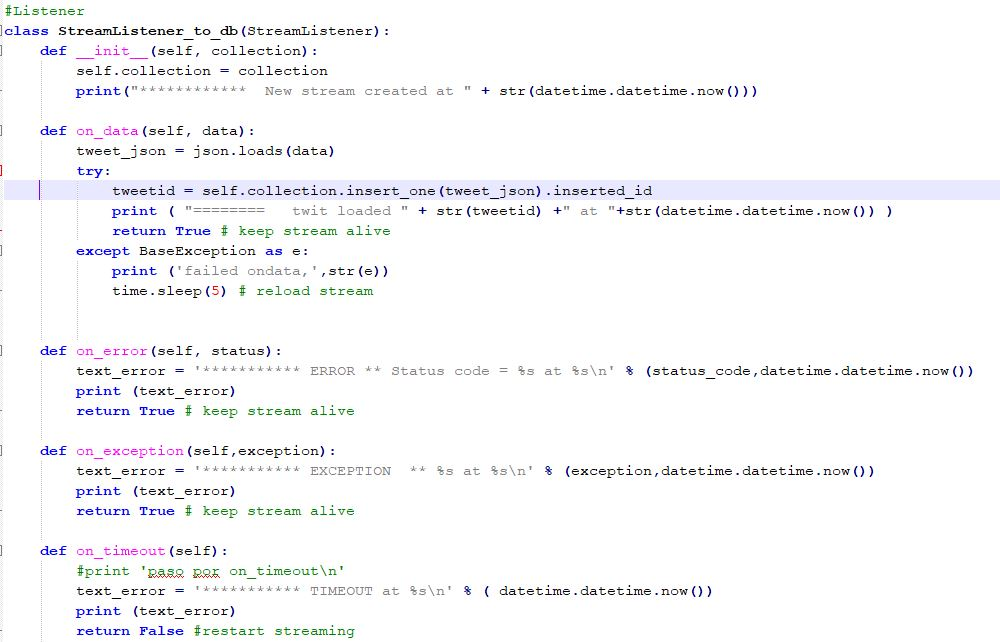
\includegraphics[width=0.6\textwidth]{streamlistener1}%
\figcaption{Función de escucha de tuits.}
\label{fig:streamlistener1} }

Para mantener vivo el proceso de escucha y que no caiga frente a errores o timeouts,
incluimos en el script un control de incidencias:

\myfigure{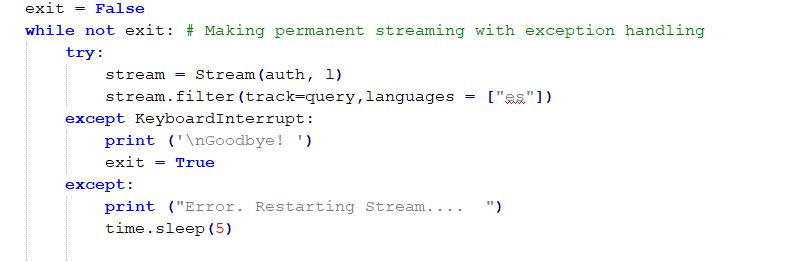
\includegraphics[width=0.6\textwidth]{streamlistener2}%
\figcaption{Gestión de incidencias en el proceso de escucha.}
\label{fig:streamlistener2} }

Y para refrescar el proceso, y que la conexión con Twitter funcione correctamente
de forma continua, se programaron relanzamientos diarios del script en el programador 
de tareas de Windows.
 
\section{Lenguajes de implementación}

Para el desarrollo de la mayor parte de la lógica del proyecto hemos elegido Python 3.6 (a través de la
instalación de Anaconda). Esta elección tiene diversas ventajas, en las varias fases del proyecto, ya
que este lenguaje facilita las siguientes tareas:
\begin{itemize}
\item Comunicación con el API Streaming de Twitter a través del paquete {\tt Tweepy}.
\item Sencilla interacción con el formato JSON, que es en el que los tuits son descargados desde el API, gracias al paquete {\tt json}.
\item  Comunicación con la base de datos documental MongoDB, a través del paquete {\tt pymongo}.
\item Incorporación nativa del encoding UTF-8 (\lq\lq Unicode Transformation Format\rq\rq con números de 8 bits), 
lo que nos ahorra muchos quebraderos de cabeza al tratar con caracteres especiales del español (tildes, ñ, etc.)
y la presencia de emojis en los textos de los tuits.\footnote{\url{https://docs.python.org/3/howto/unicode.html. }}
\end{itemize}


\section{Almacenamiento y manipulación de los datos}
Para la primera toma de contacto con los datos descargados del API de Twitter, nos hemos decantado por almacenarlos según íbamos recogiéndolos en una base de datos MongoDB. Las razones son varias:
\begin{itemize}
\item MongoDB trata de forma natural documentos en formato JSON.
\item También maneja sin problemas documentos con encoding UTF-8\footnote{
\url{https://docs.mongodb.com/v3.4/reference/bson-types/ }}, lo que nos ayuda a no tener problemas de encoding al
almacenar los tuits.
\item Se integra muy bien en programas en Python gracias al paquete {\tt pymongo}.
\item No necesita una definición de la estructura del documento, lo que es muy conveniente
para tratar tuits, donde el número de campos que obtenemos del API y el contenido de esos campos no siempre
sigue el mismo formato. Este punto es en particular relevante si el API de Twitter cambiase, o se introdujeran nuevos 
campos. Por ejemplo: a partir del 26 de Septiembre de 2017,  Twitter cambió el límite de 140 caracteres
a un límite de 280 caracteres a algunos usuarios, y eso provocó que aparecieran nuevos campos en el cuerpo de cada
tuit\footnote{\url{https://developer.twitter.com/en/docs/tweets/tweet-updates }}.
\item Es una base de datos bastante rápida, y escalable.
\end{itemize}
